\chapter{Analyse et spécification des besoins}

\section{Introduction}
Ce deuxième chapitre couvre le sprint préparatoire, étape qui
précède la réalisation incrémentale. J'y identifie les acteurs du
système, je formalise les besoins fonctionnels et non fonctionnels,
je dresse le diagramme de cas d'utilisation global, j'organise le
management Scrum (rôles, Product Backlog, planification des
sprints), je trace l'architecture globale de l'application et je
décris l'environnement de développement. Ce sprint préparatoire
pose toutes les fondations qui rendent possible la réalisation
incrémentale du produit dans les chapitres suivants.

\section{Spécification des besoins}

\subsection{Identification des acteurs}
Quatre acteurs principaux interagissent avec \nova. Pour chacun, je
précise son rôle, son mode d'authentification et la nature de ses
interactions avec le système.

\paragraph{Administrateur de l'entreprise.}
L'administrateur est l'utilisateur payant qui s'inscrit sur la
plateforme. Dans une clinique mono-médecin, il est aussi le médecin~;
dans une configuration multi-praticiens, il est typiquement un
médecin senior ou un gestionnaire administratif~; dans un
laboratoire, il est le biologiste responsable~; dans un garage, il
est le chef mécanicien. Il configure les services, ajoute les
membres d'équipe, définit les heures de travail, approuve les
campagnes proposées par le moteur d'intelligence et pilote
l'activité depuis le tableau de bord. Son authentification repose
sur un lien magique envoyé par e-mail via Supabase Auth~: aucun mot
de passe n'est stocké et les politiques Row-Level Security
s'appuient sur \texttt{auth.uid()} pour restreindre l'accès au seul
périmètre de l'administrateur connecté.

\paragraph{Praticien (membre d'équipe).}
Le praticien est un médecin, un biologiste, un mécanicien ou un
coiffeur rattaché à une entreprise. Ses permissions sont
volontairement plus restreintes que celles de l'administrateur~: il
voit sa journée, ses patients et son historique, mais pas les
tableaux financiers ni la gestion d'équipe. Il s'authentifie via le
même lien magique, et son rôle est croisé avec les politiques RLS
(via la colonne \texttt{auth\_uid} de la table \texttt{users}) pour
limiter sa visibilité aux seules ressources de son périmètre.

\paragraph{Patient ou client.}
Le patient (ou client, dans les verticaux non médicaux) est
l'utilisateur final. Il interagit avec \nova{} principalement via
WhatsApp~: il envoie des demandes de rendez-vous, pose des questions
FAQ, envoie des photos de prescriptions ou de pièces de voiture, et
répond aux rappels. Certains patients vont plus loin et installent
la PWA \nova{} sur leur téléphone, ce qui leur donne accès à une
expérience plus riche (position dans la file d'attente avec ETA
temps réel, check-in QR à la clinique, chronologie de fichiers,
profil). Côté WhatsApp, l'identité du patient est établie par son
numéro de téléphone vérifié par Meta. Côté PWA, une vérification
supplémentaire par OTP à six chiffres est imposée pour fusionner
ses historiques de visites.

\paragraph{Système (agents automatisés).}
Le quatrième acteur est le système lui-même, considéré comme un
acteur externe à part entière. Plusieurs fonctionnalités
s'exécutent selon une planification \texttt{cron} plutôt qu'en
réponse à une action utilisateur~: les rappels 24~h et 1~h, le
scan quotidien de remplissage de créneaux, le batch d'anniversaire
qui génère les vouchers, la revue hebdomadaire d'apprentissage des
durées, la campagne de réactivation des clients dormants. Ces
agents s'exécutent dans Supabase Edge Functions avec la clé de
service qui contourne intentionnellement les politiques RLS puisque
les agents agissent au nom du système et non d'un utilisateur.

\subsection{Besoins fonctionnels}
Les besoins fonctionnels sont exprimés sous forme de \emph{user
stories} (US) regroupées par acteur. Chaque story suit la
formulation~: \og En tant que <acteur>, je peux <action>, afin de
<bénéfice attendu>. \fg{}

\paragraph{Administrateur.}
\begin{itemize}[leftmargin=1.5em,itemsep=2pt,topsep=2pt]
  \item \textbf{US01} -- En tant qu'administrateur, je peux m'inscrire avec email et lien magique, afin de créer mon profil d'entreprise.
  \item \textbf{US02} -- Je peux choisir un type d'entreprise, afin de bénéficier de valeurs par défaut sectorielles.
  \item \textbf{US03} -- Je peux ajouter et gérer mes services, afin de tenir mon catalogue à jour.
  \item \textbf{US04} -- Je peux ajouter et gérer les membres de mon équipe, afin que chacun ait son agenda.
  \item \textbf{US05} -- Je peux configurer le réceptionniste IA, afin d'aligner \nova{} avec mon activité.
  \item \textbf{US06} -- Je peux visualiser le calendrier, afin de piloter ma journée.
  \item \textbf{US07} -- Je peux créer, modifier et annuler manuellement un rendez-vous.
  \item \textbf{US08} -- Je peux consulter l'historique complet de chaque client.
  \item \textbf{US09} -- Je peux recevoir des notifications navigateur en temps réel.
  \item \textbf{US10} -- Je peux configurer les campagnes de vouchers d'anniversaire.
  \item \textbf{US11} -- Je peux approuver les campagnes de remplissage de créneaux.
  \item \textbf{US12} -- Je peux activer l'auto-ajustement de durée par service.
  \item \textbf{US13} -- Je peux scanner les codes QR patients depuis le tableau de bord.
  \item \textbf{US14} -- Je peux consulter le dossier médical du patient.
  \item \textbf{US15} -- Je peux gérer les véhicules (garage).
  \item \textbf{US16} -- Je peux générer le code QR de réception du laboratoire.
\end{itemize}

\paragraph{Praticien.}
\begin{itemize}[leftmargin=1.5em,itemsep=2pt,topsep=2pt]
  \item \textbf{US17} -- En tant que praticien, je peux voir mes rendez-vous de la journée dans la PWA.
  \item \textbf{US18} -- Je peux marquer un patient comme \emph{Arrivé} ou \emph{Terminé}.
  \item \textbf{US19} -- Je peux scanner un QR patient avec mon téléphone.
  \item \textbf{US20} -- Je peux cliquer sur \emph{Terminer Consultation} à la fin de la visite.
\end{itemize}

\paragraph{Patient ou client.}
\begin{itemize}[leftmargin=1.5em,itemsep=2pt,topsep=2pt]
  \item \textbf{US21} -- En tant que patient, je peux envoyer un message WhatsApp dans l'une des trois langues.
  \item \textbf{US22} -- Je peux réserver un rendez-vous via une conversation multi-tour.
  \item \textbf{US23} -- Je peux confirmer ou annuler un rendez-vous via les boutons interactifs.
  \item \textbf{US24} -- Je peux envoyer un document attaché à mon dossier.
  \item \textbf{US25} -- Je peux envoyer la photo des dégâts de ma voiture.
  \item \textbf{US26} -- Je peux scanner le QR de réception du laboratoire.
  \item \textbf{US27} -- Je peux voir ma position et l'ETA dans la file d'attente.
  \item \textbf{US28} -- Je peux recevoir un voucher WhatsApp le jour de mon anniversaire.
  \item \textbf{US29} -- Je peux installer la PWA \nova{} et la consulter hors ligne.
  \item \textbf{US30} -- Je peux vérifier mon numéro via un OTP à six chiffres.
\end{itemize}

\paragraph{Système (agents automatisés).}
\begin{itemize}[leftmargin=1.5em,itemsep=2pt,topsep=2pt]
  \item \textbf{US31} -- En tant que système, j'envoie les rappels 24~h avec boutons Confirmer/Annuler.
  \item \textbf{US32} -- J'envoie les rappels 1~h avant le rendez-vous.
  \item \textbf{US33} -- Je détecte chaque matin les créneaux vides et crée des brouillons de campagne.
  \item \textbf{US34} -- J'exécute le batch d'anniversaire chaque matin et génère les vouchers.
  \item \textbf{US35} -- Je recalcule les durées de service chaque semaine.
  \item \textbf{US36} -- Je réactive les clients dormants par campagne hebdomadaire.
  \item \textbf{US37} -- Je traite l'auto-redemption d'un voucher.
  \item \textbf{US38} -- J'auto-attache les photos reçues au véhicule correspondant.
\end{itemize}

\subsection{Besoins non fonctionnels}
\begin{itemize}
  \item \textbf{Sécurité.} Row-Level Security multi-locataire,
        secrets hors dépôt dans les variables d'environnement des
        fonctions Edge, OTP hachés SHA-256 salés avant stockage,
        HTTPS imposé sur toutes les surfaces.
  \item \textbf{Fiabilité.} Un appel IA défaillant ne doit jamais
        bloquer la prise de rendez-vous~: le message entrant est
        toujours persisté avant l'appel à Claude, et un timeout
        strict de six secondes garantit qu'un service externe lent
        ne propage pas sa latence à l'utilisateur final.
  \item \textbf{Pertinence.} Les prompts incluent le catalogue de
        services réel du locataire pour éviter les hallucinations~;
        un jeu de tests d'évaluation tourne avant chaque release.
  \item \textbf{Scalabilité.} L'architecture est nativement
        \emph{stateless} côté fonctions Edge~; Supabase auto-scale
        son pool Postgres~; les crons s'exécutent via
        \texttt{pg\_cron} dans la base, sans worker externe.
  \item \textbf{Mises à jour temps réel.} Les tuiles du tableau de
        bord et les positions de file d'attente se mettent à jour
        en moins de deux secondes via Supabase Realtime.
  \item \textbf{Support multilingue.} Arabe dialectal, français et
        anglais en messages entrants, réponses sortantes, gabarits
        de vouchers et textes de rappel.
  \item \textbf{Mobile-first.} La PWA est entièrement
        fonctionnelle sur téléphones jusqu'à 360~px de largeur~; le
        tableau de bord redirige automatiquement les administrateurs
        mobiles vers la PWA.
  \item \textbf{Fenêtre de réponse de cinq secondes.} L'IA doit
        répondre en moins de cinq secondes pour 95\,\% des cas.
  \item \textbf{Conformité RGPD.} Les numéros de téléphone et
        conversations sont attachés à l'entreprise concernée et
        supprimables sur demande.
  \item \textbf{Maîtrise des coûts.} Le coût total d'infrastructure
        par locataire et par mois doit rester sous 5~USD en régime
        de croisière.
\end{itemize}

\subsection{Diagramme de cas d'utilisation global}
Le diagramme de cas d'utilisation global, figure~\ref{fig:uc},
positionne les quatre acteurs et les principales fonctionnalités
qu'ils invoquent. Il sert de socle aux raffinements par sprint qui
seront déclinés dans les chapitres de réalisation.

% ===========================================================================
% Diagramme de cas d'utilisation global — Nova AI
% ===========================================================================
\begin{figure}[H]
\centering
\begin{tikzpicture}[
  font=\footnotesize,
  every node/.style={align=center},
  actor/.style ={font=\footnotesize\bfseries},
  uc/.style    ={ellipse, draw=black!75, fill=cyan!8,
                 minimum width=32mm, minimum height=8mm,
                 font=\scriptsize, inner sep=2pt},
  inc/.style   ={->, thick, draw=black!70, dashed, >=Stealth},
  rel/.style   ={-, thick, draw=black!75},
  sys/.style   ={rectangle, draw=black!60, fill=white,
                 minimum width=88mm, minimum height=110mm,
                 line width=1pt}
]

% System box (Nova AI)
\node[sys] (sys) at (0,0) {};
\node[font=\bfseries, anchor=north] at (sys.north) {\bfseries Système Nova~AI};

% Use-case nodes inside the system, arranged in two columns
% Left column — patient flow
\node[uc] (book)     at (-2.0, 4.2) {Réserver un\\rendez-vous};
\node[uc] (cancel)   at (-2.0, 3.0) {Annuler un\\rendez-vous};
\node[uc] (resched)  at (-2.0, 1.8) {Reprogrammer\\un rendez-vous};
\node[uc] (uploadrx) at (-2.0, 0.6) {Envoyer une\\ordonnance};
\node[uc] (askinfo)  at (-2.0,-0.6) {Demander des\\informations};
\node[uc] (urgent)   at (-2.0,-1.8) {Signaler une\\urgence};

% Right column — staff flow
\node[uc] (viewcal)  at ( 2.0, 4.2) {Consulter le\\calendrier};
\node[uc] (mngsvc)   at ( 2.0, 3.0) {Gérer les\\services};
\node[uc] (mngteam)  at ( 2.0, 1.8) {Gérer l'équipe};
\node[uc] (revenue)  at ( 2.0, 0.6) {Voir les\\indicateurs};
\node[uc] (asknova)  at ( 2.0,-0.6) {Interroger Nova\\(vocal)};
\node[uc] (settings) at ( 2.0,-1.8) {Configurer\\horaires \& IA};

% Shared
\node[uc] (auto-ai)  at ( 0.0,-3.4) {Classifier l'intention\\(IA)};

% Actors outside the system
\node[actor]                                 (patient) at (-7.5, 1.5) {\faUser\ Patient};
\node[actor, font=\footnotesize\bfseries]    (owner)   at ( 7.5, 2.5) {Propriétaire\\(médecin / gérant)};
\node[actor, font=\footnotesize\bfseries]    (recept)  at ( 7.5,-0.5) {Réceptionniste\\/ assistant};
\node[actor, font=\footnotesize\bfseries]    (system)  at ( 0.0,-5.0) {\textit{<<système IA>>}\\Anthropic Claude};

% Patient relationships
\draw[rel] (patient) -- (book);
\draw[rel] (patient) -- (cancel);
\draw[rel] (patient) -- (resched);
\draw[rel] (patient) -- (uploadrx);
\draw[rel] (patient) -- (askinfo);
\draw[rel] (patient) -- (urgent);

% Owner relationships
\draw[rel] (owner) -- (viewcal);
\draw[rel] (owner) -- (mngsvc);
\draw[rel] (owner) -- (mngteam);
\draw[rel] (owner) -- (revenue);
\draw[rel] (owner) -- (asknova);
\draw[rel] (owner) -- (settings);

% Receptionist subset
\draw[rel] (recept) -- (book);
\draw[rel] (recept) -- (resched);
\draw[rel] (recept) -- (viewcal);

% AI inclusion
\draw[inc] (book)    -- node[midway, sloped, above=-1pt, font=\tiny]{<<include>>} (auto-ai);
\draw[inc] (askinfo) -- node[midway, sloped, above=-1pt, font=\tiny]{<<include>>} (auto-ai);
\draw[inc] (urgent)  -- node[midway, sloped, above=-1pt, font=\tiny]{<<include>>} (auto-ai);
\draw[inc] (asknova) -- node[midway, sloped, above=-1pt, font=\tiny]{<<include>>} (auto-ai);
\draw[rel] (system)  -- (auto-ai);

\end{tikzpicture}
\caption{Diagramme de cas d'utilisation global : trois acteurs humains (patient, propriétaire, réceptionniste) interagissent avec le système, qui s'appuie sur l'acteur secondaire \textit{<<système IA>>} Anthropic Claude pour classifier les intentions et conduire les conversations multi-tours.}
\label{fig:uc}
\end{figure}


\subsection{Diagramme de classes global}
Le diagramme de classes global, figure~\ref{fig:class-global}, modélise
les entités persistantes du domaine \nova{} et leurs associations.
Les classes centrales sont \texttt{Business} (locataire),
\texttt{User} (membre d'équipe), \texttt{Client} (patient ou client
final), \texttt{Service} (catalogue), \texttt{Appointment}
(rendez-vous), \texttt{Message} (conversation WhatsApp),
\texttt{Notification} (alertes temps réel) et \texttt{Document}
(pièces jointes). Les classes sectorielles \texttt{Voucher},
\texttt{Vehicle} (pack garage) et \texttt{QueueEntry} (pack
laboratoire) sont introduites par le Sprint~3 et représentées ici
pour donner la vue complète du modèle de données. Ce diagramme
sert de contrat entre la couche métier et le schéma SQL appliqué
via les migrations Supabase.

% =======================================================================
% Diagramme de classes global -- source : figures/sources/class-global.puml
% Genere via https://plantuml.com/plantuml/uml -> export PNG -> figures/class-global.png
% =======================================================================
\begin{figure}[!htbp]\centering
\IfFileExists{figures/class-global.png}{%
  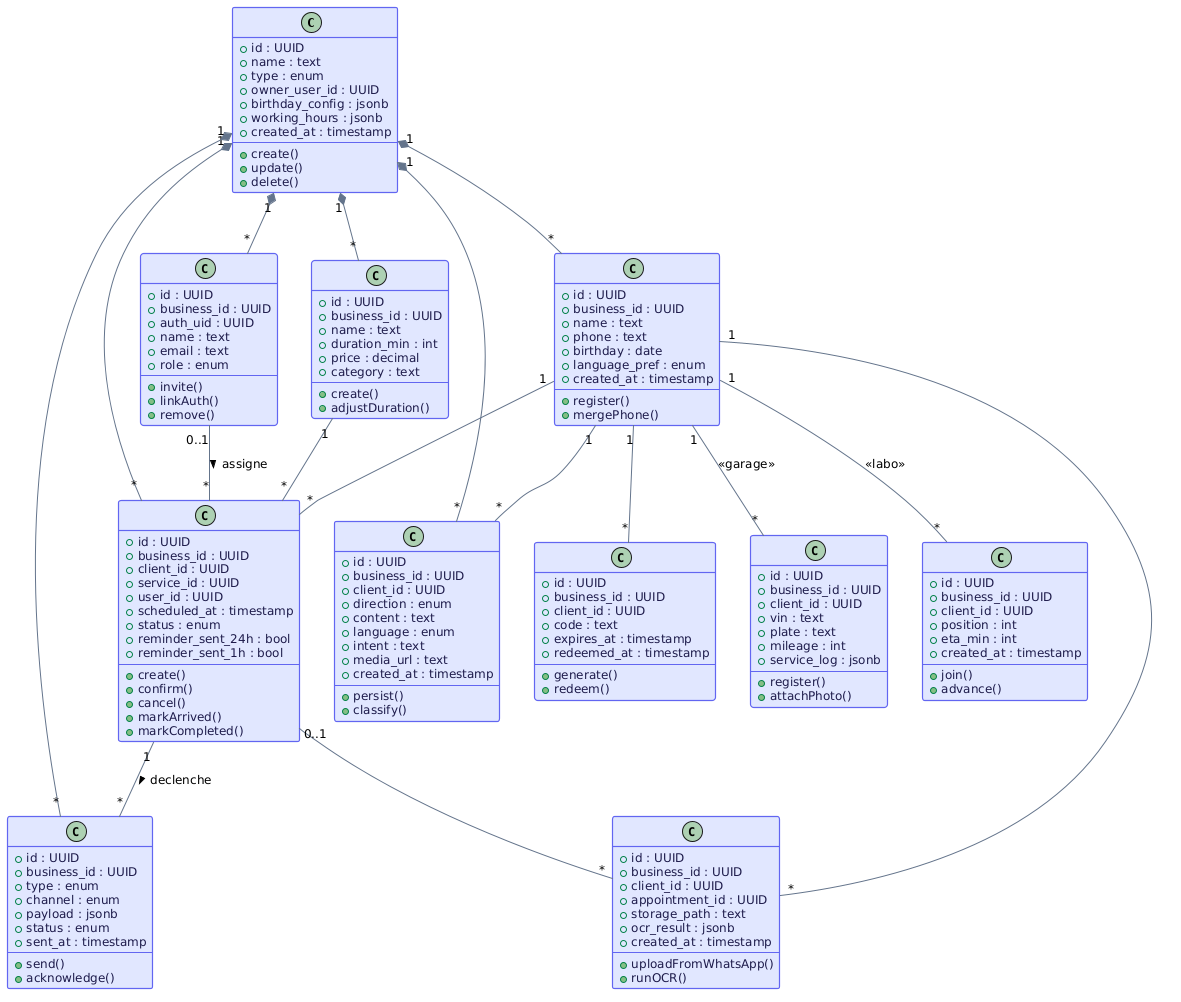
\includegraphics[width=.98\textwidth,height=.88\textheight,keepaspectratio]{figures/class-global.png}%
}{%
  \fbox{\parbox[c][7cm][c]{0.85\textwidth}{\centering\itshape\small
    [Diagramme de classes global -- a generer depuis\\
    \texttt{figures/sources/class-global.puml} via\\
    \url{https://www.plantuml.com/plantuml/uml}\\
    puis sauvegarder en \texttt{figures/class-global.png}]
  }}%
}
\caption{Diagramme de classes global de \nova{}.}
\label{fig:class-global}
\end{figure}

\section{Management du projet Scrum}

\subsection{Rôles et responsabilités}
J'ai adapté l'organisation Scrum à la réalité d'un projet mené par
un développeur unique avec une encadrante. Les rôles se
répartissent comme suit~:
\begin{itemize}
  \item \textbf{Développeur} -- \textbf{MEHDI CHEIKH}. Je suis
        l'auteur unique du code, du schéma de base, des fonctions
        Edge, du tableau de bord et de la PWA. Je suis responsable
        de la livraison technique de chaque sprint.
  \item \textbf{Scrum Master} -- \textbf{Mme Hana Derouiche}.
        Mon encadrante universitaire anime les revues
        hebdomadaires, valide le respect du processus et arbitre
        les priorités lorsque le backlog est en tension.
  \item \textbf{Product Owner} -- \textbf{ISMAIK}. L'institut, en
        tant qu'organisme d'accueil, porte la vision produit, fixe
        le cadre du PFE et valide la pertinence des besoins
        identifiés sur le terrain.
\end{itemize}

\subsection{Product Backlog}
Le Product Backlog consolide mes trente-huit \emph{user stories} en
une liste priorisée. La priorité est exprimée sur trois niveaux~:
\textbf{P1} (indispensable première démo bout-en-bout), \textbf{P2}
(indispensable pour un locataire en production), \textbf{P3}
(différenciateur qui enrichit l'expérience).

{\small
\begin{longtable}{|p{1.6cm}|p{1.4cm}|p{1.4cm}|p{8.5cm}|}
  \caption{Product Backlog -- User Stories.}\label{tab:backlog}\\
  \hline\hline
  \textbf{Acteur} & \textbf{ID} & \textbf{Prio} & \textbf{User story (résumé)} \\
  \hline
  \endfirsthead
  \multicolumn{4}{l}{\small\textit{Tableau \ref{tab:backlog} (suite)}}\\
  \hline\hline
  \textbf{Acteur} & \textbf{ID} & \textbf{Prio} & \textbf{User story} \\
  \hline
  \endhead
  \hline
  \multicolumn{4}{r}{\small\textit{(suite page suivante)}}\\
  \endfoot
  \hline\hline
  \endlastfoot
  Admin     & US01 & P1 & Inscription email + lien magique. \\
  \hline
  Admin     & US02 & P1 & Choix du type d'entreprise. \\
  \hline
  Admin     & US03 & P1 & Gestion des services. \\
  \hline
  Admin     & US04 & P2 & Gestion de l'équipe. \\
  \hline
  Admin     & US05 & P1 & Configuration du réceptionniste IA. \\
  \hline
  Admin     & US06 & P1 & Visualisation du calendrier. \\
  \hline
  Admin     & US07 & P1 & Création / modification manuelle d'un RDV. \\
  \hline
  Admin     & US08 & P2 & Historique complet d'un client. \\
  \hline
  Admin     & US09 & P2 & Notifications temps réel. \\
  \hline
  Admin     & US10 & P3 & Campagnes vouchers anniversaire. \\
  \hline
  Admin     & US11 & P3 & Approbation des campagnes Demand-Fill. \\
  \hline
  Admin     & US12 & P3 & Auto-ajustement de durée. \\
  \hline
  Admin     & US13 & P2 & Scan QR du tableau de bord. \\
  \hline
  Admin     & US14 & P3 & Consultation du dossier médical. \\
  \hline
  Admin     & US15 & P3 & Gestion des véhicules. \\
  \hline
  Admin     & US16 & P3 & QR de réception laboratoire. \\
  \hline
  Praticien & US17 & P2 & Vue PWA des RDV du jour. \\
  \hline
  Praticien & US18 & P2 & Marquer Arrivé / Terminé. \\
  \hline
  Praticien & US19 & P3 & Scan QR mobile. \\
  \hline
  Praticien & US20 & P2 & Bouton Terminer Consultation. \\
  \hline
  Patient   & US21 & P1 & Conversation WhatsApp multilingue. \\
  \hline
  Patient   & US22 & P1 & Réservation multi-tour. \\
  \hline
  Patient   & US23 & P2 & Confirmer / annuler via boutons. \\
  \hline
  Patient   & US24 & P3 & Envoi de document. \\
  \hline
  Patient   & US25 & P3 & Envoi photo dégâts voiture. \\
  \hline
  Patient   & US26 & P3 & Scan QR de réception. \\
  \hline
  Patient   & US27 & P3 & Position file d'attente. \\
  \hline
  Patient   & US28 & P3 & Voucher anniversaire WhatsApp. \\
  \hline
  Patient   & US29 & P2 & Installation PWA hors ligne. \\
  \hline
  Patient   & US30 & P2 & Vérification OTP. \\
  \hline
  Système   & US31 & P1 & Rappels 24~h. \\
  \hline
  Système   & US32 & P2 & Rappels 1~h. \\
  \hline
  Système   & US33 & P3 & Scan quotidien Demand-Fill. \\
  \hline
  Système   & US34 & P3 & Batch anniversaire. \\
  \hline
  Système   & US35 & P3 & Apprentissage hebdomadaire des durées. \\
  \hline
  Système   & US36 & P3 & Réactivation des clients dormants. \\
  \hline
  Système   & US37 & P3 & Auto-redemption voucher. \\
  \hline
  Système   & US38 & P3 & Auto-attache photos garage. \\
\end{longtable}
}

\subsection{Planification des sprints}
J'ai découpé le backlog en quatre sprints. Le sprint préparatoire
correspond à la phase d'analyse (le présent chapitre). Les sprints
1, 2 et 3 portent la réalisation incrémentale du produit.

\begin{table}[H]
  \centering\small
  \caption{Planification des sprints.}
  \label{tab:plan}
  \renewcommand{\arraystretch}{1.45}
  \begin{tabular}{|p{2.6cm}|>{\raggedright\arraybackslash}p{1.6cm}|>{\raggedright\arraybackslash}p{2.6cm}|>{\raggedright\arraybackslash}p{6.4cm}|}
    \hline\hline
    \textbf{Sprint} & \textbf{Durée} & \textbf{Période} & \textbf{Description} \\
    \hline
    Sprint préparatoire & 3 sem. & Février--mars 2026 & Analyse et préparation : spécification des besoins, conception UML globale, choix techniques, environnement de développement. \\
    \hline
    Sprint 1 & 3 sem. & Mars 2026 & Fondations : schéma multi-locataire, RLS, authentification, webhook WhatsApp, classifieur IA. \\
    \hline
    Sprint 2 & 3 sem. & Avril 2026 & Surfaces opérationnelles : tableau de bord administrateur, gestion des rendez-vous et clients, OCR documents, PWA patient. \\
    \hline
    Sprint 3 & 4 sem. & Avril--mai 2026 & Couche d'intelligence : remplissage de créneaux, apprentissage des durées, vouchers d'anniversaire, packs sectoriels, voix. \\
    \hline\hline
  \end{tabular}
\end{table}

La figure~\ref{fig:gantt} synthétise ce découpage sous la forme
d'une frise verticale qui aligne chaque sprint sur le calendrier,
de la phase d'analyse jusqu'à la soutenance.

% =======================================================================
% Frise verticale -- source : figures/sources/gantt.mmd (flowchart TB)
% Regenerer le PNG sur https://mermaid.live apres modification.
% =======================================================================
\begin{figure}[!htbp]\centering
\IfFileExists{figures/gantt.png}{%
  \includegraphics[width=.55\textwidth,height=.88\textheight,keepaspectratio]{figures/gantt.png}%
}{%
  \fbox{\parbox[c][12cm][c]{0.55\textwidth}{\centering\itshape\small
    [Frise verticale de la planification -- a generer depuis\\
    \texttt{figures/sources/gantt.mmd} via \url{https://mermaid.live}\\
    puis sauvegarder en \texttt{figures/gantt.png}]
  }}%
}
\caption{Planification des sprints de \nova{} sous forme de frise verticale.}
\label{fig:gantt}
\end{figure}

\section{Environnement de développement}

\subsection{Environnement matériel}
J'ai développé le projet sur mon poste de travail personnel,
complété par des terminaux de test pour valider l'expérience
mobile et la PWA.

\begin{table}[H]
  \centering\small
  \caption{Environnement matériel utilisé pour la réalisation du projet.}
  \label{tab:hw}
  \renewcommand{\arraystretch}{1.4}
  \begin{tabular}{|p{4.2cm}|>{\raggedright\arraybackslash}p{9cm}|}
    \hline\hline
    \textbf{Équipement} & \textbf{Caractéristiques} \\
    \hline
    Poste de développement & Ordinateur portable Intel Core~i5, 8 à 16~Go de RAM, SSD~NVMe, écran Full~HD. \\
    \hline
    Tablette de test & Tablette Android pour vérifier le \emph{responsive} intermédiaire. \\
    \hline
    Smartphone Android & Test de WhatsApp Cloud API, installation PWA, notifications push. \\
    \hline
    Smartphone iOS & Vérification du rendu Safari mobile et compatibilité service worker. \\
    \hline
    Connexion Internet & Fibre domestique pour le codage, partage 4G de secours pour les revues à distance. \\
    \hline\hline
  \end{tabular}
\end{table}

\subsection{Environnement logiciel}
Le tableau~\ref{tab:tools} synthétise les outils et services que
j'ai utilisés.

{\small
\renewcommand{\arraystretch}{1.4}
\begin{longtable}{|m{1.9cm}|>{\raggedright\arraybackslash}m{4.5cm}|>{\raggedright\arraybackslash}m{6.4cm}|}
  \caption{Pile logicielle : outils, fonctionnalités et justification.}\label{tab:tools}\\
  \hline\hline
  \textbf{Outil} & \textbf{Fonctionnalités utilisées} & \textbf{Justification du choix} \\
  \hline
  \endfirsthead
  \multicolumn{3}{l}{\small\textit{Tableau \ref{tab:tools} (suite)}}\\
  \hline\hline
  \textbf{Outil} & \textbf{Fonctionnalités utilisées} & \textbf{Justification du choix} \\
  \hline
  \endhead
  \hline
  \multicolumn{3}{r}{\small\textit{(suite page suivante)}}\\
  \endfoot
  \hline\hline
  \endlastfoot
  \includegraphics[width=1.7cm,height=0.9cm,keepaspectratio]{figures/logos/supabase.png}
    & Postgres, Auth lien magique, Storage, Edge Functions, Realtime, RLS.
    & Stack tout-en-un cohérent, RLS native qui simplifie le multi-locataire. \\
    \hline
  \includegraphics[width=1.7cm,height=0.9cm,keepaspectratio]{figures/logos/postgres.png}
    & Schéma relationnel, JSONB, contraintes CHECK, triggers, vues matérialisées.
    & Maturité éprouvée, écosystème \texttt{pg\_cron} / \texttt{pg\_net}. \\
    \hline
  \includegraphics[width=1.7cm,height=0.9cm,keepaspectratio]{figures/logos/deno.png}
    & Runtime des fonctions Edge Supabase.
    & Cold-start faible, TypeScript natif, distribution mondiale. \\
    \hline
  \includegraphics[width=1.7cm,height=0.9cm,keepaspectratio]{figures/logos/claude.png}
    & Claude Haiku pour la classification, Claude Sonnet pour l'OCR.
    & Meilleur ratio vitesse/coût sur le JSON structuré. \\
    \hline
  \includegraphics[width=1.7cm,height=0.9cm,keepaspectratio]{figures/logos/whatsapp.png}
    & API Cloud WhatsApp Business, messages, médias, boutons.
    & Canal dominant en Tunisie, API directe sans agrégateur. \\
    \hline
  \includegraphics[width=1.7cm,height=0.9cm,keepaspectratio]{figures/logos/vercel.png}
    & Hébergement statique du tableau de bord et de la PWA.
    & Déploiement en moins de 30~s, HTTPS gratuit, CDN mondial. \\
    \hline
  \includegraphics[width=1.7cm,height=0.9cm,keepaspectratio]{figures/logos/openai.png}
    & Whisper pour la transcription des notes vocales WhatsApp.
    & Support natif de l'arabe et du français. \\
    \hline
  \includegraphics[width=1.7cm,height=0.9cm,keepaspectratio]{figures/logos/elevenlabs.png}
    & Clonage et synthèse vocale.
    & Qualité naturelle élevée, API simple à intégrer. \\
    \hline
  \includegraphics[width=1.7cm,height=0.9cm,keepaspectratio]{figures/logos/twilio.png}
    & Webhook voix téléphonique optionnel.
    & Numéros virtuels régionaux, API documentée. \\
    \hline
  \includegraphics[width=1.7cm,height=0.9cm,keepaspectratio]{figures/logos/n8n.png}
    & Orchestration d'automatismes annexes.
    & Interface visuelle, déclencheurs cron faciles. \\
    \hline
  \includegraphics[width=1.7cm,height=0.9cm,keepaspectratio]{figures/logos/html5qrcode.png}
    & Décodage QR côté client.
    & Léger, sans serveur, fonctionne hors ligne. \\
    \hline
  \includegraphics[width=1.7cm,height=0.9cm,keepaspectratio]{figures/logos/vscode.png}
    & Éditeur principal pour TypeScript, SQL, HTML, LaTeX.
    & Intégration Git native, riche en extensions. \\
    \hline
  \includegraphics[width=1.7cm,height=0.9cm,keepaspectratio]{figures/logos/git.png}
    & Gestion de versions locale.
    & Standard de l'industrie, branchement léger. \\
    \hline
  \includegraphics[width=1.7cm,height=0.9cm,keepaspectratio]{figures/logos/github.png}
    & Dépôt distant, déclencheurs Vercel, journal des releases.
    & Intégration Vercel sans configuration. \\
    \hline
  \includegraphics[width=1.7cm,height=0.9cm,keepaspectratio]{figures/logos/plantuml.png}
    & Génération des diagrammes UML (séquence, cas d'utilisation).
    & Code source versionnable, rendu reproductible. \\
    \hline
  \includegraphics[width=1.7cm,height=0.9cm,keepaspectratio]{figures/logos/mermaid.png}
    & Diagrammes complémentaires.
    & Syntaxe lisible directement dans le code. \\
    \hline
  \includegraphics[width=1.7cm,height=0.9cm,keepaspectratio]{figures/logos/overleaf.png}
    & Édition collaborative en ligne du rapport LaTeX.
    & Compilation cloud sans installer de distribution locale. \\
    \hline
  \includegraphics[width=1.7cm,height=0.9cm,keepaspectratio]{figures/logos/latex.png}
    & Composition du rapport.
    & Rendu typographique académique standard. \\
\end{longtable}
}

\section{Architecture globale de l'application}
\nova{} suit une architecture en trois plans empilés
verticalement~: les \textbf{frontends} (le tableau de bord
administrateur et la PWA patient), le \textbf{backend} Supabase
(base PostgreSQL avec Row-Level Security, authentification,
stockage, moteur temps réel et fonctions Edge), et les
\textbf{services externes} (Meta WhatsApp Cloud API, Anthropic
Claude pour l'IA, OpenAI Whisper pour la transcription audio,
ElevenLabs pour la voix). La figure~\ref{fig:nova-archi} en donne
une vue synthétique avec les liaisons entre les trois couches.

\paragraph{Frontends.}
Deux applications monopages distinctes constituent les surfaces
utilisateurs~: (i) le \emph{tableau de bord administrateur}
(\texttt{/}), destiné au desktop et à la tablette, et (ii) la
\emph{PWA patient} (\texttt{/pwa/}), destinée au mobile. Les deux
sont écrites en JavaScript ES~Modules vanille, sans framework ni
étape de \emph{build}, et sont servies en statique depuis Vercel.

\paragraph{Backend.}
Le backend est un projet Supabase qui rassemble une base Postgres
avec Row-Level Security, un service d'authentification (Auth) à
lien magique, un stockage (Storage) compatible S3, un moteur
temps réel (Realtime) qui pousse les changements de tables aux
clients abonnés, et un runtime Edge Functions (Deno) qui héberge le
webhook WhatsApp et les automatismes (\texttt{classify-message},
\texttt{send-reminders}, \texttt{demand-fill-runner}).

\paragraph{Liaison frontend / backend.}
Les frontends communiquent exclusivement avec le backend via deux
canaux~: (1)~PostgREST sur HTTPS pour les requêtes SQL transformées
en API REST, signées par le JWT issu d'Auth et contraintes par les
politiques RLS, et (2)~WebSockets pour les abonnements Realtime
(\texttt{postgres\_changes}). Aucune logique métier critique ne vit
côté frontend~: toutes les règles sensibles (insertion d'un
rendez-vous, attribution d'un token de check-in, hachage des OTP)
sont appliquées soit par des contraintes SQL, soit par des fonctions
Edge.

% Schema technique detaille de l'architecture
% =======================================================================
% Architecture globale Nova AI -- vue verticale en 3 couches
% =======================================================================
% Source : figures/sources/nova-archi.mmd (Mermaid)
% Image generee verticale (portrait), taille reduite pour partager la
% page avec le texte descriptif.
% =======================================================================
\begin{figure}[!htbp]\centering
\IfFileExists{figures/nova-archi.png}{%
  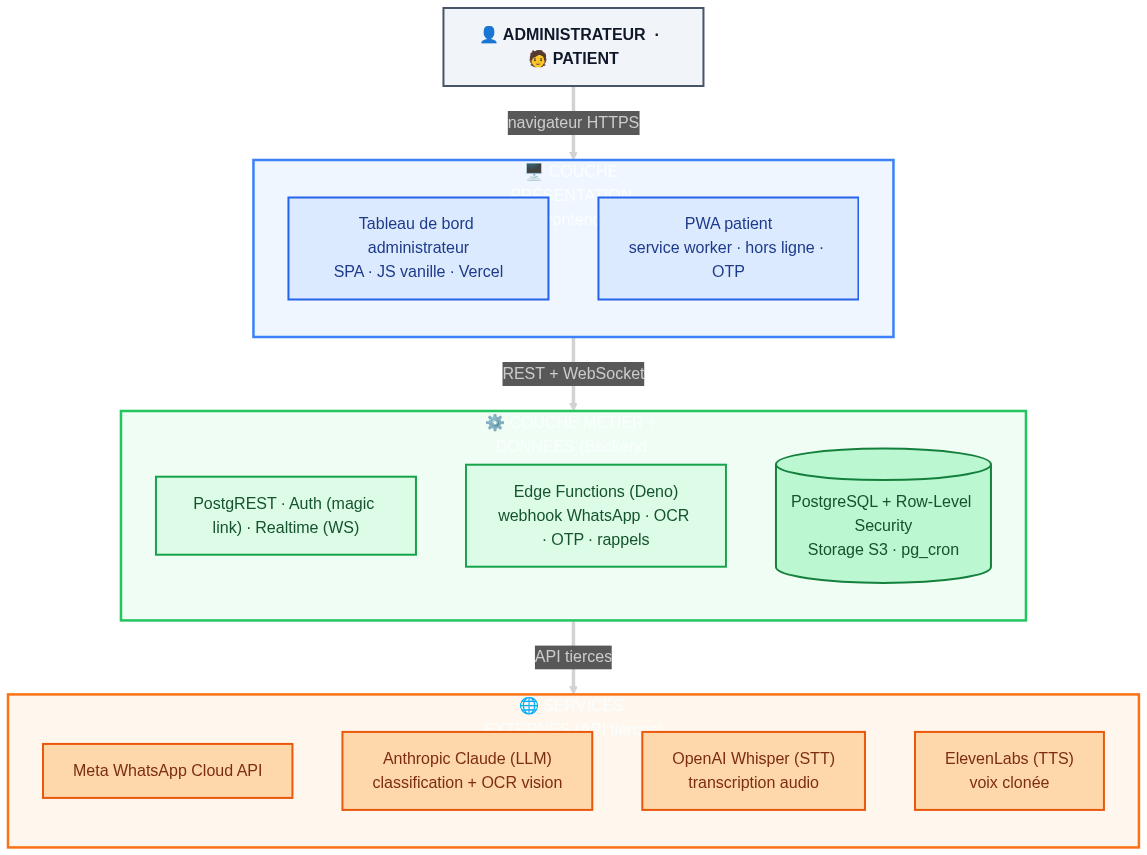
\includegraphics[width=.72\textwidth,height=1.0\textheight,keepaspectratio]{figures/nova-archi.png}%
}{%
  \fbox{\parbox[c][8cm][c]{0.42\textwidth}{\centering\itshape\small
    [Architecture globale (vue verticale) -- a generer depuis\\
    \texttt{figures/sources/nova-archi.mmd} via\\
    \url{https://mermaid.live} puis sauvegarder en\\
    \texttt{figures/nova-archi.png}]
  }}%
}
\caption{Architecture globale de \nova{} : trois couches empilées verticalement -- frontends, backend Supabase, services externes.}
\label{fig:nova-archi}
\end{figure}


\section{Conclusion}
Ce chapitre a posé les spécifications, le management Scrum, la
planification, l'environnement de développement et l'architecture
globale de \nova. Les trois chapitres suivants entrent dans le
détail de chaque sprint de réalisation~: \textbf{Sprint~1} pour les
fondations, \textbf{Sprint~2} pour les surfaces opérationnelles et
\textbf{Sprint~3} pour la couche d'intelligence.
